\subsubsection{UC2 - Visualizzazione errore autenticazione}\label{UC2}

\begin{figure}[H]
  \centering
  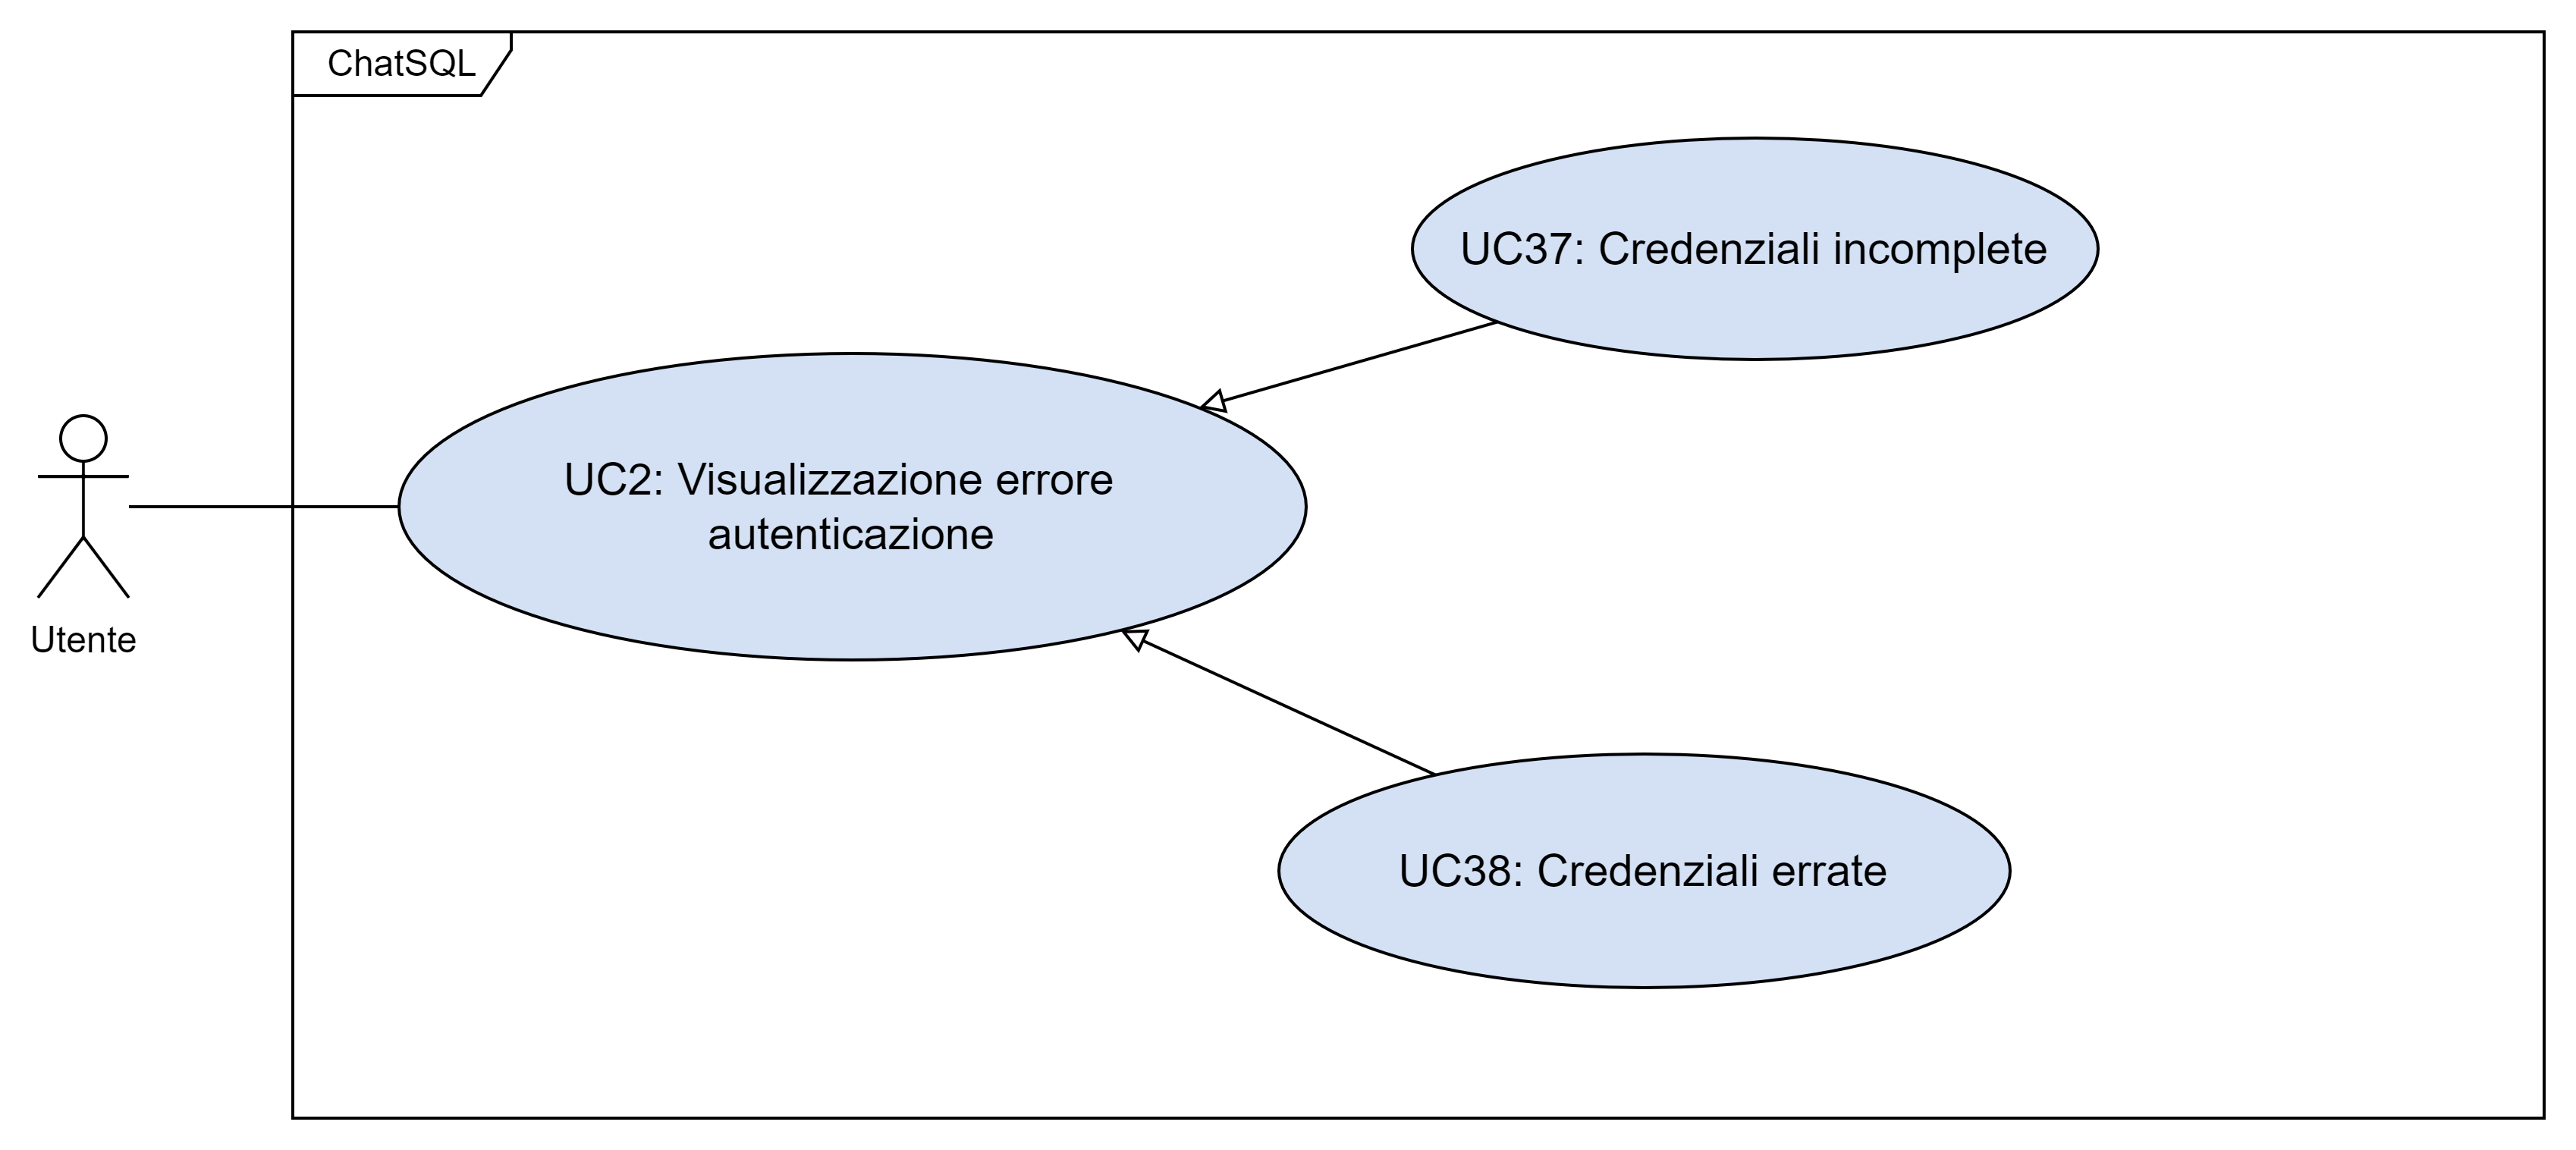
\includegraphics[width=0.90\textwidth]{assets/uc2.png}
  \caption{UC2}
\end{figure}

\paragraph*{Descrizione}
Nel caso in cui il sistema rilevi delle irregolarità durante la validazione delle credenziali, l'Utente viene informato della natura del problema tramite un apposito messaggio di errore.

\paragraph*{Attori principali}
Utente

\paragraph*{Precondizioni}
\begin{itemize}
  \item Il sistema è attivo e funzionante;
  \item L'Utente ha inserito le proprie credenziali nell'area di login (\hyperref[UC1]{UC1});
  \item Il sistema ha riscontrato un problema nel processo di autenticazione.  
\end{itemize}

\paragraph*{Postcondizioni}
\begin{itemize}
  \item Viene visualizzato un messaggio d'errore esplicativo.
\end{itemize}

\paragraph*{Scenario principale}
\begin{enumerate}
  \item L'Utente tenta di autenticarsi inserendo le proprie credenziali nell'area di login;
  \item Il sistema riscontra un problema nella validazione delle credenziali di accesso;
  \item Viene restituito all'Utente un messaggio di errore;
  \item Il sistema invita l'Utente a riprovare l'autenticazione.
\end{enumerate}

\paragraph*{Specializzazioni}
\begin{itemize}
  \item Credenziali incomplete (\hyperref[UC37]{UC37});
  \item Credenziali errate (\hyperref[UC38]{UC38}).
\end{itemize}

%%%%%%%%%%%%%%%%%%%%%%%%%%%%%%%%%%%%%%%%%%%%%%%%%%%%%%%%%%%%%%%%%%%%%%%%%%%%%%

\subsubsection{UC2.1 - Credenziali incomplete}\label{UC2point1}
\paragraph*{Descrizione}
Il sistema restituisce un messaggio di errore qualora l'Utente inserisca delle credenziali incomplete in fase di autenticazione.

\paragraph*{Attori principali}
Utente

\paragraph*{Precondizioni}
\begin{itemize}
  \item L'Utente ha inserito credenziali incomplete;
  \item L'Utente ha richiesto l'autenticazione. 
\end{itemize}

\paragraph*{Postcondizioni}
\begin{itemize}
  \item Viene visualizzato un messaggio di errore esplicativo.
\end{itemize}

\paragraph*{Scenario principale}
\begin{enumerate}
  \item L'Utente richiede l'autenticazione inserendo credenziali incomplete;
  \item La procedura di autenticazione fallisce;
  \item L'Utente visualizza un messaggio con i dettagli dell'errore.
\end{enumerate}

%%%%%%%%%%%%%%%%%%%%%%%%%%%%%%%%%%%%%%%%%%%%%%%%%%%%%%%%%%%%%%%%%%%%%%%%%%%%%%

\subsubsection{UC2.2 - Credenziali errate}\label{UC2point2}
\paragraph*{Descrizione}
Il sistema restituisce un messaggio di errore qualora l'Utente inserisca delle credenziali non valide in fase di autenticazione.

\paragraph*{Attori principali}
Utente

\paragraph*{Precondizioni}
\begin{itemize}
  \item L'Utente ha inserito credenziali errate;
  \item L'Utente ha richiesto l'autenticazione. 
\end{itemize}

\paragraph*{Postcondizioni}
\begin{itemize}
  \item Viene visualizzato un messaggio di errore esplicativo.
\end{itemize}

\paragraph*{Scenario principale}
\begin{enumerate}
  \item L'Utente richiede l'autenticazione inserendo credenziali errate; 
  \item Il sistema non riconosce le credenziali fornite;  
  \item La procedura di autenticazione fallisce;
  \item L'Utente visualizza un messaggio con i dettagli dell'errore.
\end{enumerate}